\documentclass{article}
\usepackage{graphicx} % Required for inserting images
\usepackage{babel}
\usepackage{enumitem}
\usepackage{float}
\usepackage{chngcntr}
\usepackage{glossaries}
\usepackage{tabularx}
\usepackage{hyperref}
\usepackage{titletoc}
\usepackage{titlesec}
\usepackage{csquotes}
\usepackage{pgf-pie}   
\usepackage{glossaries-extra}
\usepackage{pdfpages}
\counterwithin{figure}{section}
\counterwithin{table}{section}
\setlength\parindent{0pt}

\title{User Manual \\
        Discrete Choice Model Builder}
\date{}
\begin{document}
\maketitle
\thispagestyle{empty}
\newpage
\startcontents[maintableofcontents]
\printcontents[maintableofcontents]{}{1}[2]{\section*{Table of Contents}}
\thispagestyle{empty}
\newpage
\pagenumbering{arabic}

\newpage
\section{The Program's graphical Interface}
\begin{figure}[H]% 
  \centering
  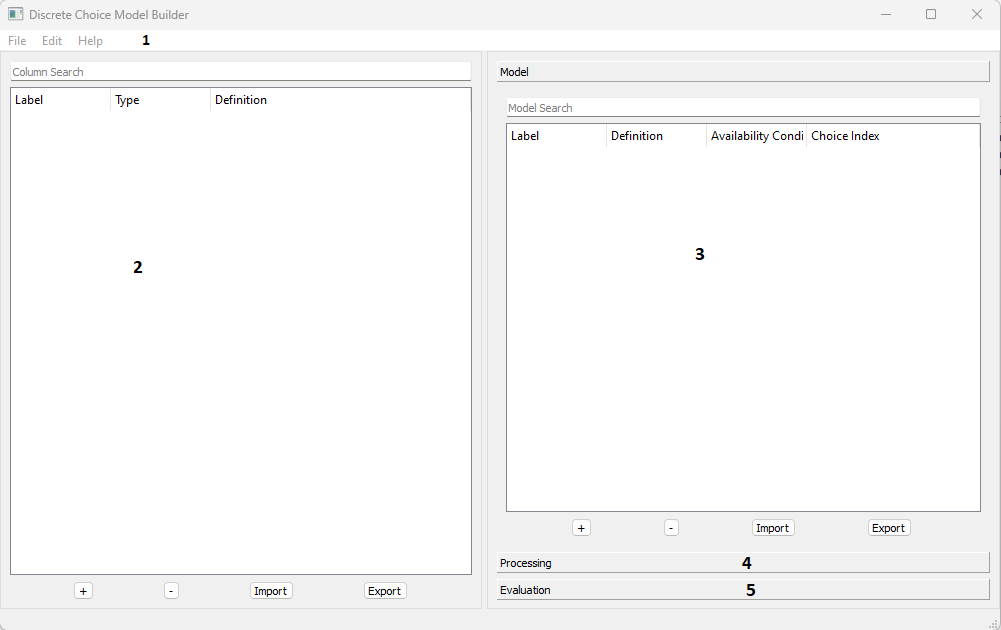
\includegraphics[width=15cm]{docs/User Manual/img/GUI.png}
  \caption{The GUI}
  \label{fig:gui}
\end{figure} 
\begin{enumerate} [label=\textbf{\arabic*})]
    \item This is the menu bar. In covers three menus. File menu, Edit menu and Help menu. Further information can be found in \ref{sec:menus}.
    \item This part of the GUI is the column widget,where the columns of the survey data are displayed. The derivativesare also shon here. Detailed discription is found in \ref{sec:columns}.
    \item The Model widget the alternatives (aka utility functions) can be added and modified. Further information are in section \ref{sec:model}.
    \item The Processing Widget is where the processing method can be chosen. To expand this widget, click on the "Processing" bar as shown in figure \ref{fig:gui}. Consider visiting section \ref{sec:processing} for more information.
    \item The Evaluation Widget is where the model can be evaluated and the results are displayed. To expand this widget, click on the "Evaluation" bar as shown in figure \ref{fig:gui}. Detailed discription is in \ref{sec:evaluation}.
\end{enumerate}
\subsection{The Menus} \label{sec:menus}
\subsubsection{File Menu}
\begin{figure}[H]% 
  \centering
  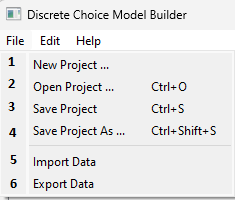
\includegraphics[width=6cm]{docs/User Manual/img/File Menu.png}
  \caption{The File Menu}
  \label{fig:filemenu}
\end{figure}
\begin{enumerate} [label=\textbf{\arabic*})]
    \item Opens an empty project.
    \item Opens an existing project. For that you need the path of the project's folder. A project can contain derivatives, alternatives, processing information, survey data and an evaluation.
    \item Saves the current project in a pre-chosen path. The user will be requested for the path if none exists.
    \item Allows saving the project in a different path under a different name.
    \item This button is for importing survey data from a chosen path. It's only possible to import one CSV file.
    \item Export data means the survey data as well as the derivatives will be exported to a path of your choice as a CSV file.
\end{enumerate}
\subsubsection{Edit Menu}
\begin{figure}[H]% 
  \centering
  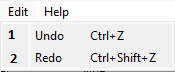
\includegraphics[width=4cm]{docs/User Manual/img/Edit Menu.png}
  \caption{The Edit Menu}
  \label{fig:editmenu} 
\end{figure}
\begin{enumerate} [label=\textbf{\arabic*})]
    \item With Undo you can reverse the last change.
    \item With Redo you can reset the last Undo.
\end{enumerate}
\subsubsection{Help Menu}
\begin{figure}[H]% 
  \centering
  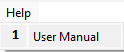
\includegraphics[width=3cm]{docs/User Manual/img/Help menu.png}
  \caption{The Help Menu}
  \label{fig:helpmenu} 
\end{figure}
\begin{enumerate} [label=\textbf{\arabic*})]
    \item Opens the user manual.
\end{enumerate}
\newpage
\subsection{The Column Widget} \label{sec:columns}
This is where names of the columns from the imported survey data are displayed. Even the derivatives are shown here.
\begin{figure}[H]% 
  \centering
  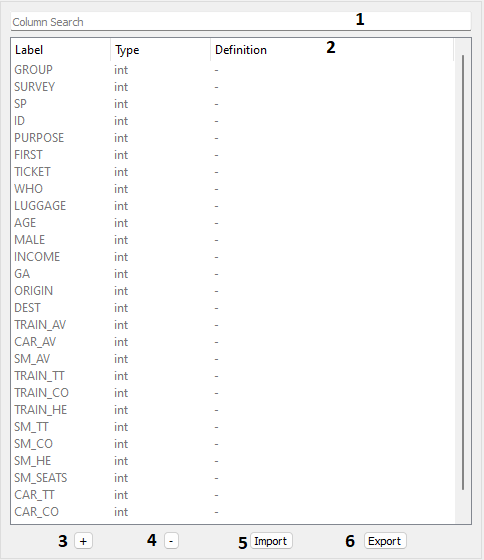
\includegraphics[width=8cm]{docs/User Manual/img/ColumnWidget.png}
  \caption{The Columns table}
  \label{fig:columns} 
\end{figure}
\begin{enumerate} [label=\textbf{\arabic*})]
    \item Using this search bar, it's possible to search for columns and derivatives using their labels.
    \item The table is divided into three columns. Label stands for name of a derivative or a column from the imported CSV file, which contains the survey data. Type indicates the possible type of the derivative or the data, which are stored under the corrosponding label in the survey data. Definition is only available for a derivative. This is where you can see its definition (As a function).
    \item This button is for adding a new derivative. A new window appears, where you can enter the derivative. It's possible to modify a  derivative after adding it by clicking twice on the cell to modify. \\
    \newpage
    \begin{figure}
        \centering
        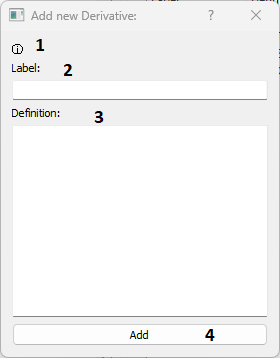
\includegraphics[width=5cm]{docs/User Manual/img/newDervNew.png}
        \caption{Window to add a Derivative}
        \label{fig:enter-label}
    \end{figure} \\
    
    \begin{enumerate} [label=\textbf{\arabic*})]
        \item  Hovering over this circle will show you the syntax specification for label and definition.
        \item Label stands for the name of the derivative.
        \item The syntax for the definition is python syntax. This includes mathematical and logical expressions with or without varibales. 
        \item Click the button for confirmation and to add the derivative.
    \end{enumerate} \\
    \item If you click on a derivative and then on the "-" button, the chosen derivative will get deleted.
    \item This is used to import an external derivative. Note that only JSON files can be accepted.
    \item Choose derivatives from the table and then click on the "Export" button to export the derivatives to a path of your choice.
\end{enumerate}
\newpage
\subsection{The Model Table} \label{sec:model}
\begin{figure}[H]% 
  \centering
  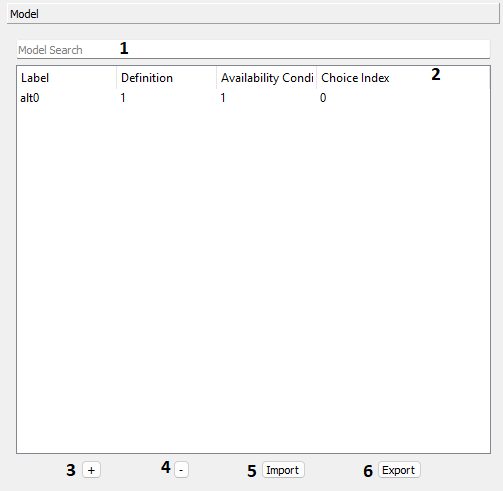
\includegraphics[width=9cm]{docs/User Manual/img/ModelWidget.png}
  \caption{The Model}
  \label{fig:model} 
\end{figure}
\begin{enumerate} [label=\textbf{\arabic*})]
    \item In this search bar it's possible to search for an alternative using its label.
    \item The table in this widget consists of 4 columns: label for the names of the alternatives,  definition for the functions, availability condition indicates when the alternative should be considered, and choice index to identify and sort the alternatives. Please note that an alternative with choice index equal to 0 must be defined.
    \item This button will open a new window, where you can define a new alternative to add it to the table. \\
    \newpage
    \begin{figure}
        \centering
        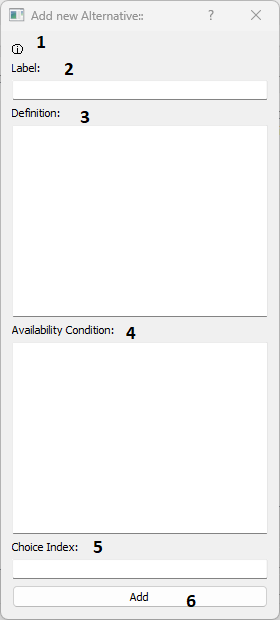
\includegraphics[width = 4cm]{docs/User Manual/img/newAltNew.png}
        \caption{Add Alternative Window}
        \label{fig:adAlt}
    \end{figure} \\
    \begin{enumerate}[label=\textbf{\arabic*})]
        \item The syntax for the definition of alternatives is the same as Python syntax. This includes mathematical and logical expressions. If you hover over this circle, you will find specific information regarding the syntax.
        \item The label of the alternative.
        \item The definition of the alternative.
        \item The availaibility condition of the alternative.
        \item The choice index of the alternative.
        \item The button to confirm and add a new alternative.
    \end{enumerate}
    \item This button deletes alternatives after choosing them.
    \item It's possible to import. Currently only JSON files can be imported.
    \item This button enables exporting alternatives after choosing them from the table. The alternatives will be exported as JSON files to path of your choice.
\end{enumerate}
\newpage
\subsection{The Processing Widget} \label{sec:processing}
\begin{figure}[H]% 
  \centering
  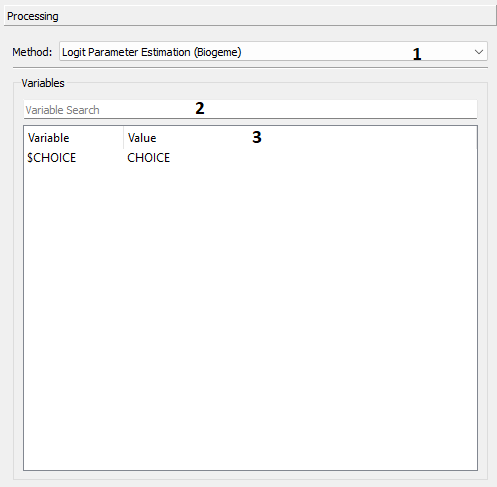
\includegraphics[width=9cm]{docs/User Manual/img/Processing.png}
  \caption{The Processing Widget}
  \label{fig:processing} 
\end{figure}
\begin{enumerate} [label=\textbf{\arabic*})]
    \item Here you can choose the processing method. \\
    \begin{figure}[H]% 
        \centering
        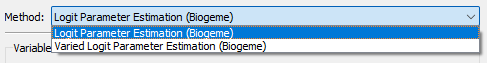
\includegraphics[width=9cm]{docs/User Manual/img/Processing method.png}
        \caption{The Processing Methods}
        \label{fig:processingmethods} 
    \end{figure}
    \item This search bar is useful if you want to search for a specific variable in the table.
    \item The variable called '\$Choice' represents the value that defines in the data what Alternative was chosen.
    \item The table shows all parameters found in the derivatives that can be varied. Here you can put in values you want to calculate the model for. These parameters are the ones that change when the model is updated.
\end{enumerate}
\newpage
\subsection{The Evaluation Widget} \label{sec:evaluation}
\begin{figure}[H]% 
  \centering
  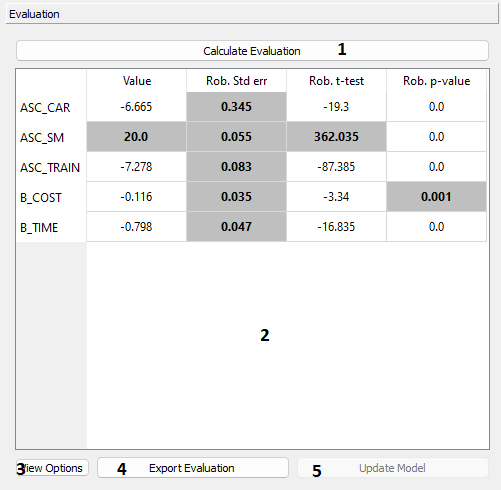
\includegraphics[width=9cm]{docs/User Manual/img/newEval.png}
  \caption{The Evaluation Widget}
  \label{fig:evaluation} 
\end{figure}
\begin{enumerate} [label=\textbf{\arabic*})]
    \item This button is to start the evaluation process. During the evaluation it's not possible to use the program. Instead wait until the calculation finishes.
    \item In the table the evaluation is displayed. Some cells are highlighted, because the values in these cells are above the thresholds.
    \item This button will open a new window, where you can adjust the thresholds to highlight cells in the table. \\
    \newpage
    \begin{figure}[H]% 
        \centering
        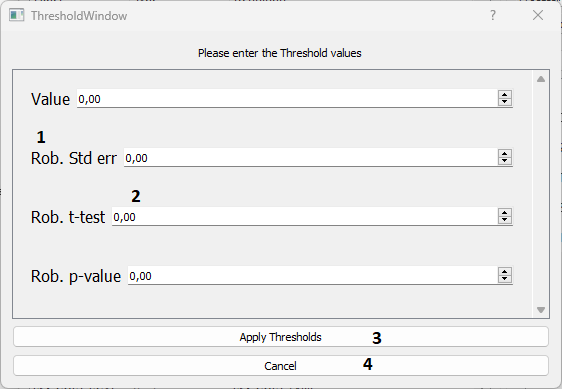
\includegraphics[width=9cm]{docs/User Manual/img/thresholdWindow.png}
        \caption{The Threshold Window}
        \label{fig:thresholds} 
    \end{figure} \\
    \begin{enumerate} [label=\textbf{\arabic*})]
        \item This stands for the name of the column in the evaluation table.
        \item In this field you can enter a threshold for a specifc column.
        \item This button is for confirming changes and applying the thresholds
        \item The "Cancel" button will close the window without applying the new thresholds.
    \end{enumerate}
    \item Using this button it's possible to export the results as a CSV-file.
    \item The feature to optimize the model is unavailable in the current version.
\end{enumerate}
\newpage
\section{Displaying Errors}
There are two ways to display errors in the program:
\begin{enumerate} [label=\arabic*.]
    \item Using marker to display syntax errors. To see the details and causes of an error, hover over the faulty cell. \\
    \begin{figure} [H]
        \centering
        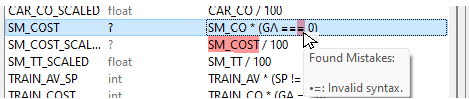
\includegraphics[width = 8 cm]{docs/User Manual/img/marker.png}
        \caption{Error Marker}
        \label{fig:marker}
    \end{figure}
    \item Using notification windows. For example when performing the evaluation, but an exception is thrown during the calculation. In the notification window the cause for an unsuccessful calculation is displayed.
    \begin{figure} [H]
        \centering
        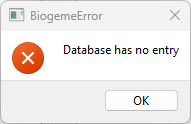
\includegraphics[width = 5 cm]{docs/User Manual/img/exception.png}
        \caption{Notification Window with Explanation}
        \label{fig:exception}
    \end{figure}
\end{enumerate}
\end{document}